\documentclass{report}
\usepackage[utf8]{inputenc}
\usepackage[italian]{babel}
\usepackage[linktoc=all]{hyperref}
\usepackage{graphicx}
\hypersetup{
	colorlinks,
	citecolor=black,
	filecolor=black,
	linkcolor=black,
	urlcolor=black
}
\usepackage[a4paper,includeheadfoot,margin=2.54cm]{geometry}
\usepackage{fancyhdr}

\pagestyle{fancy}
\fancyhf{}
\rhead{Economia}
\lhead{\leftmark}
\rfoot{\thepage}

\renewcommand{\chaptermark}[1]{%
	\markboth{#1}{}}

\begin{document}
	
	\author{Davide Parpinello}
	\title{%
			\begin{Large}
				Appunti di\\
			\end{Large}
		Economia ed Innovazione d'Impresa}
	\date{Luglio 2019}
	\maketitle
	
	\tableofcontents
	
	\chapter{Introduzione all'economia}
	\section{Il problema economico}
	Il problema economico fondamentale è la scarsità: le risorse a disposizione non sono mai sufficienti a soddisfare tutti i bisogni degli agenti economici.
	Questo implica l'esigenza di operare scelte. L'economia studia quindi le scelte degli agenti economici per gestire le risorse scarse e le regole e/o istituzioni per renderle migliori.
	\section{Input e output}
	Ogni società effettua scelte relative agli input: beni/servizi utilizzati e agli output: beni/servizi risultanti dai processi produttivi.
	\section{Gli economisti studiano..}
	\begin{itemize}
		\item Le scelte individuali: come gli agenti prendono decisioni mossi dal proprio self interest
		\item L'interazione tra gli agenti sul mercato
		\item Il sistema economico e il suo funzionamento nel complesso.
	\end {itemize}
	\section{Micro e macroeconomia}
	\begin{itemize}
		\item La microeconomia analizza il comportamento degli agenti e il funzionamento dei singoli mercati
		\item La marcoeconomia considera l'economia come un sistema (es. ricchezza nazionale, inflazione..)
	\end {itemize}
	L'economia nasce nel '700 con un punto di vista macro per poi capire nel 1870 che il sistema dipende dal comportamento micro.
	\section{Scelte e agenti economici}
	\begin{itemize}
		\item Scelte degli individui o famiglie: cosa e quanto consumare, dove lavorare, quanto risparmiare. \textbf{Obiettivo:} massimizzare il benessere individuale.
		\item Scelte delle imprese: cosa, quanto e come produrre; a che prezzo vendere; come farsi pubblicita'. \textbf{Obiettivo:} massimizzare il profitto.
		\item Scelte della collettivita': come aggregare le preferenze individuali per soddisfare i bisogni collettivi. \textbf{Obiettivo:} massimizzare il benessere sociale.
	\end{itemize}
	In ogni caso i principi base del comportamento sono eguali per tutti gli agenti. Tutte le scelte dipendono dagli incentivi: motivazione misurabile.
	\section{Il mercato}
	Il mercato e' l'istituzione principale dove ha luogo l'interazione economica degli agenti.\\
	Il mercato e' un gioco a somma positiva: un meccanismo che favorisce tutti i partecipanti.\\
	Il funzionamento del mercato necessita di regole.
	\section{La concorrenza}
	La concorrenza puo' essere come processo naturale o come processo economico.
	\paragraph{Concorrenza come processo naturale} 
	Visione negativa: Darwinismo sociale, principio di sopravvivenza del piu' forte. Secondo tale visione il compito della societa' e' quello di elevare l'uomo rispetto allo stato di natura quindi cercare di eliminare la concorrenza.
	\paragraph{Concorrenza come processo economico}
	Visione statica: processo che premia chi riesce a produrre al costo piu' basso.\\Visione dinamica: processo che premia chi riesce ad innovare e/o produrre il bene di qualita' migliore.\\La concorrenza e' quindi un processo positivo perche' premia il merito di produttori e accresce il benessere dei consumatori. Occorrono comunque regole, per premiare chi merita davvero.
	\section{La scelta come \textit{trade-off}}
	\textit{Trade-off}: per ottenere una cosa si deve sempre rinunciare a qualcos'altro.\\Efficienza significa che la societa' ottiene il massimo possibile dalle proprie risorse scarse.\\Equita' significa che i benefici che derivano dalle risorse di una societa' vengono distribuiti in modo giusto.\\Non e' possibile ottenere entrambe le cose: esiste quindi un \textit{trade-off} rilevante nelle scelte del \textit{policy-maker}.
	\section{Efficienza}
	Il problema dell'efficienza e' strettamente correlato con quello della scarsita' e quindi riguarda tutti gli agenti economici.\\Efficienza infatti significa ottenere il massimo beneficio dalle risorse date oppure utilizzare il minimo ammontare di risorse per ottenere un dato livello di beneficio.\\Le regole del mercato servono a consentire il raggiungimento di queste condizioni.
	\section{Il costo opportunita'}
	Cio' a cui si deve rinunciare ogni volta che si sceglie una determinata alternativa: ad esempio detenere il proprio potere d'acquisto in moneta invece che in titoli comporta la rinuncia ad un interesse.
	\section{La razionalita' in economia}
	Essere razionali significa scegliere in base a un criterio e seguirlo coerentemente. Il criterio puo' essere uno qualsiasi, ma di solito in economia si adotta il criterio di massimizzazione della soddisfazione.
	\subsection{Razionalita' come scelta al margine}
	Le variazioni marginali sono piccoli cambiamenti incrementali rispetto a una data quantita'. Gli agenti razionali prendono le decisioni confrontando costi e benefici indotti da una variazione marginale.\\Per il criterio di scelta razionale, si compie una certa azione se e solo se il beneficio e' maggiore del costo.
	\subsection{Gli individui rispondono agli incentivi}
	Un incentivo e' un qualsiasi incremento del beneficio marginale o riduzione del costo marginale di una scelta. Al contrario, un disincentivo.\\Ogni variazione di costi/benefici induce una reazione razionale degli agenti, quindi il \textit{policy-maker} puo' indurre gli agenti a modificare certi comportamenti agendo sugli incentivi.
	\section{Perche' scambiare?}
	Lo scambio consente di incrementare il benessere degli agenti attraverso la specializzazione. Lo scambio genera maggiore benessere per tutti e consente agli agenti di specializzarsi nelle attivita' che sanno svolgere meglio.
	\medskip \\
	Esistono due modi per soddisfare i bisogni di consumo:
	\begin{itemize}
		\item Scelta autarchica: si consuma solo cio' che si produce.
		\item Scelta della specializzazione e scambio: si consuma cio' che si ottiene in cambio di cio' che si e' prodotto.
	\end{itemize}
	La piu' scelta e' la seconda perche' gli agenti specializzandosi in cio' che sanno fare e scambiando con altri agenti possono migliorare il proprio benessere. Quindi per incrementare il benessere occorre passare attraverso lo scambio.
	\subsection{Da cosa dipende la specializzazione}
	Intuitivamente dipende dalle differenze nei costi di produzione, misurabili come quantita' di input necessaria per produrre un'unita' di output (senso stretto) o come quantita' di un bene a cui si deve rinunciare per produrre un'unita' in piu' di un'altro bene (costo opportunita').
	\medskip \\ Abbiamo quindi due possibili criteri alla base dello scambio: vantaggio assoluto o vantaggio comparato.
	\section{Mercato ed efficienza}
	Un'economia di mercato e' un sistema in cui gli agenti decidono liberamente cosa comprare, per chi lavorare, cosa produrre e chi assumere. L'interazione sul libero mercato degli agenti determina il massimo benessere possibile per l'intera collettivita'.
	\section{Modelli economici}
	\subsection{Modello del flusso circolare}
	Modo semplice di visualizzare le transazioni economiche che si realizzano tra gli agenti considerati, ovvero famiglie e imprese.\medskip \\Le transazioni avvengono attraverso il mercato dei beni e servizi e quello dei fattori produttivi.\medskip \\Evidenzia sia il flusso reale di beni, servizi e fattori che quello monetario di redditi e spese.
	\begin{figure}[h]
		\centering
		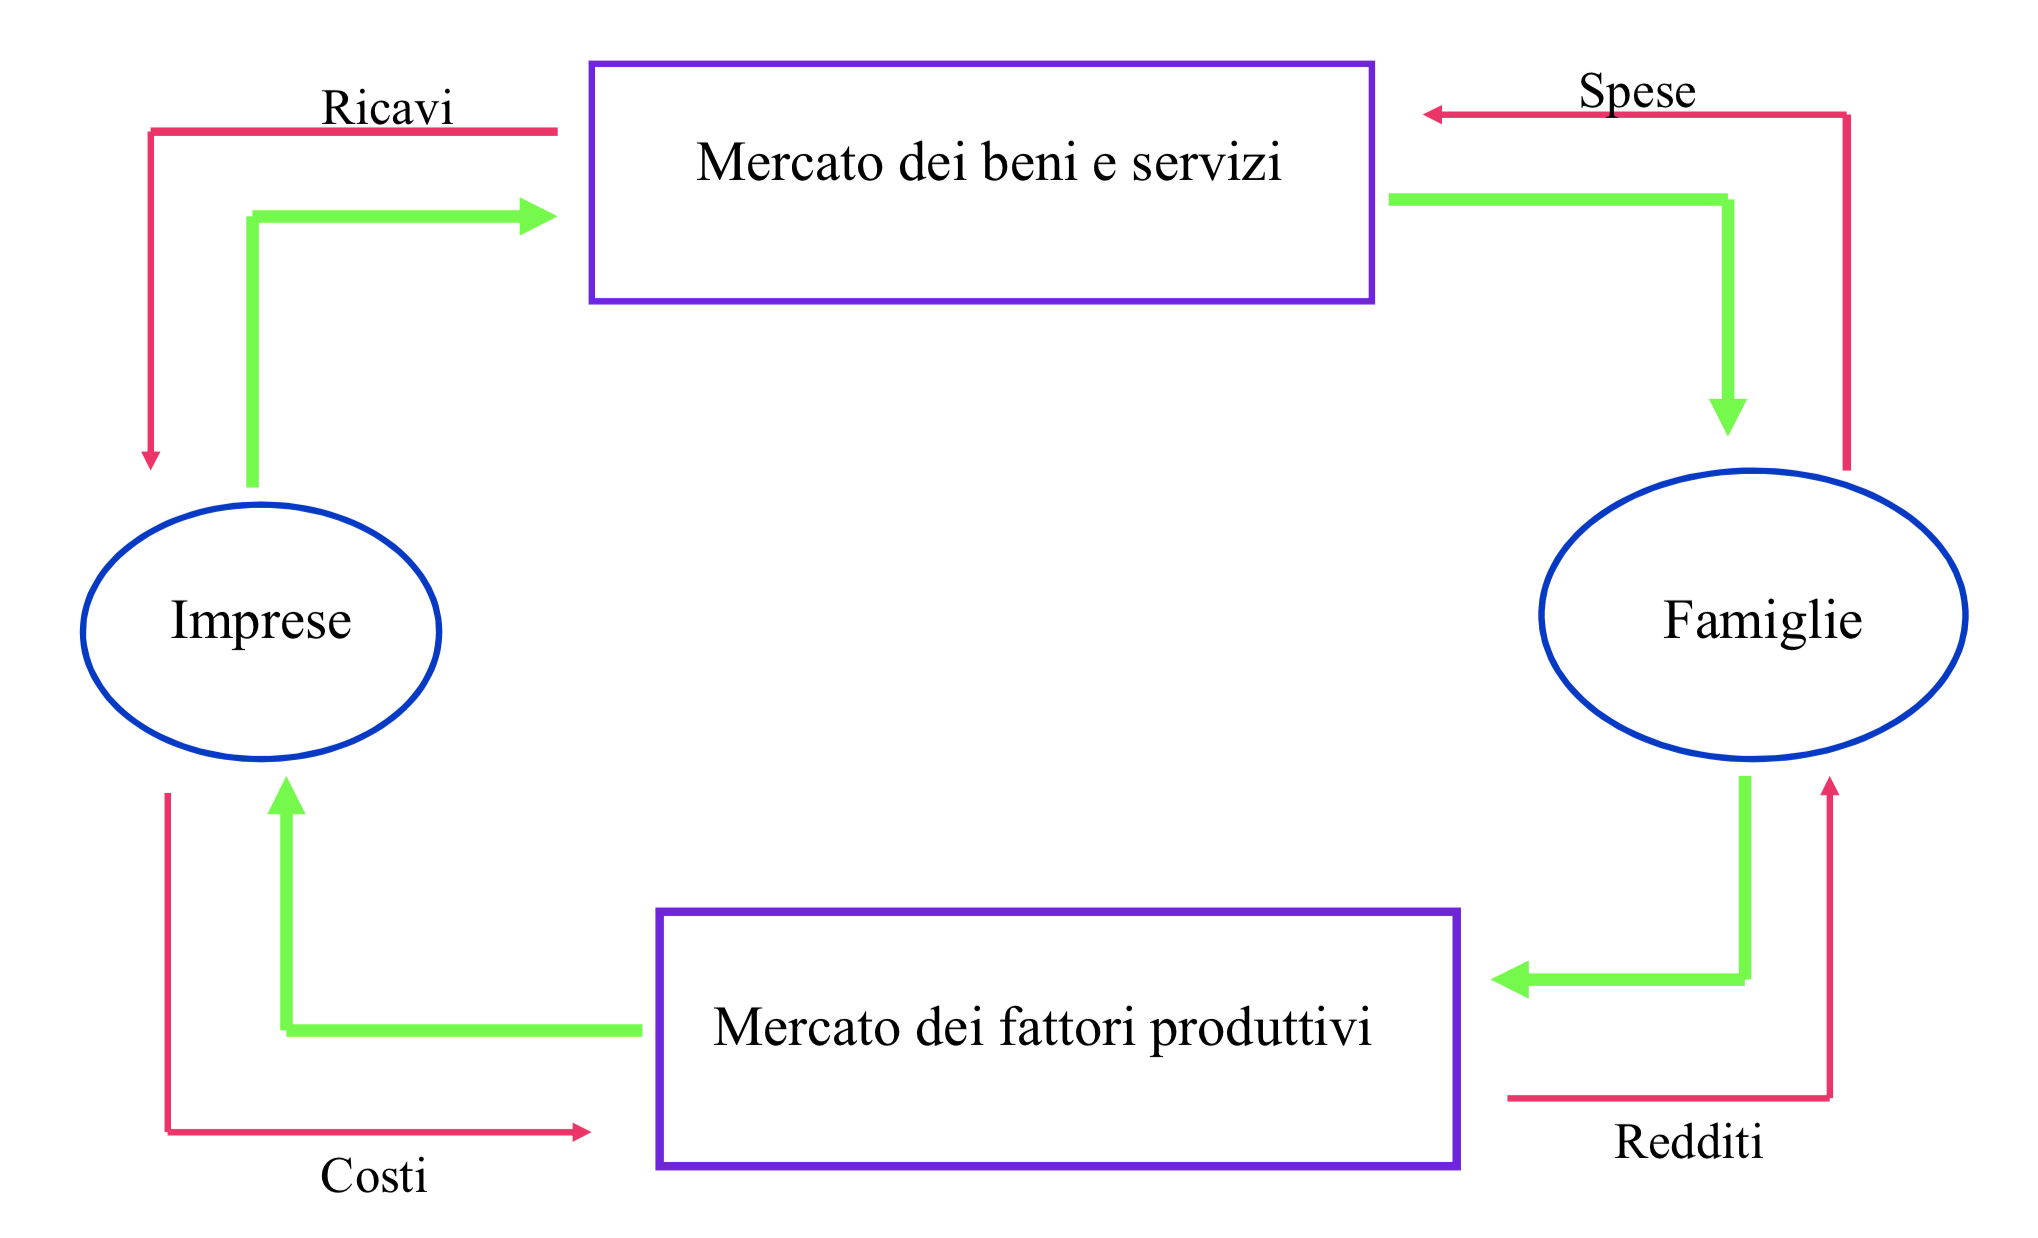
\includegraphics[width=0.7\linewidth]{flusso-circolare}
		\caption{flusso circolare}
		\label{fig:flusso-circolare}
	\end{figure}
	\subsection{Frontiera delle possibilita' di produzione}
	Illustra i \textit{trade-off} che caratterizzano un sistema economico che produce solo due beni. Mostra la quantita' massima di un bene che puo' essere prodotta, data la quantita' dell'altro bene.
	\begin{itemize}
		\item \textbf{E' decrescente}: per produrre una quantita' maggiore di un bene e' necessario sacrificare la produzione dell'altro bene;
		\item \textbf{E' concava}: all'aumentare della produzione di un bene e' necessario sacrificare quantita' sempre crescenti dell'altro bene.
	\end{itemize}
	\chapter{Il mercato}
	\large Domanda, offerta ed equilibrio
	\section{Cos'è un mercato?}
	Tema centrale della microeconomia e' lo studio del funzionamento dei mercati, ovvero insiemi regolati di compratori e venditori di beni, servizi o fattori produttivi.\medskip \\Una prima ipotesi istituzionale e' che esista sempre un prezzo positivo per il bene, quindi venditori e compratori riusciranno sempre ad accordarsi per lo scambio. Cio' implica che il mercato sia l'istituzione dove gli agenti si scambiano beni.
	\medskip \\Sono presenti 4 forme di mercato:
	\begin{itemize}
		\item Concorrenza perfetta
		\item Concorrenza monopolistica
		\item Monopolio
		\item Oligopolio
	\end{itemize}
	\section{Mercato di concorrenza perfetta}
	Vengono soddisfatte 4 ipotesi:
	\begin{enumerate}
		\item \textbf{molteplicita' e free entry:} presenti molti compratori e venditori e nessun vincolo all'ingresso nel mercato
		\item \textbf{assenza di potere di mercato:} nessun partecipante riesce a controllare prezzi o quantita'
		\item \textbf{uniformita' del prodotto:} il prodotto e' omogeneo
		\item \textbf{informazione perfetta:} tutti i partecipanti conoscono tutte le informazioni relative al mercato. Le informazioni devono essere simmetriche e complete.
	\end{enumerate}
	Da queste ipotesi discende:
	\begin{itemize}
		\item \textbf{Legge del prezzo unico:} nel mercato vige un unico prezzo
		\item \textbf{Comportamento price taking:} compratori e venditori subiscono il prezzo di mercato
	\end{itemize}
	\section{La domanda di mercato}
	\begin{itemize}
		\item La \textit{quantita' domandata} e' l'ammontare di beni che i compratori vogliono e possono acquistare
		\item La \textit{scheda di domanda} e' una tabella che mostra la relazione tra il prezzo del bene e la quantita' domandata
		\item La \textit{curva di domanda} e' la linea discendente che mette in relazione prezzo e quantita' in un sistema di assi cartesiani
	\end{itemize}
	\subsection{Le determinanti della domanda}
	La domanda di mercato dipende da diversi fattori, tra cui prezzo di mercato, reddito dei consumatori, prezzo dei beni collegati, gusti e aspettative dei consumatori.
	\medskip \\Un bene normale e' un bene la cui domanda aumenta al crescere del reddito, mentre un bene inferiore e' un bene la cui domanda, al contrario, diminuisce al crescere del reddito.
	\medskip \\Quando una diminuzione del prezzo di un bene riduce la domanda di un'altro essi si dicono sostituti, ad esempio treno e aereo; quando invece la diminuzione del prezzo di uno aumenta la domanda di un'altro vengono detti complementari.
	\section{La curva di offerta}
	\begin{itemize}
		\item La \textit{quantita' offerta} e' l'ammontare di bene che i venditori possono e vogliono vendere
		\item La \textit{scheda di offerta} e' una tabella che mostra la relazione tra il prezzo del bene e la quantita' offerta
		\item La \textit{curva di offerta} e' la linea ascendente che mette in relazione il prezzo e la quantita' offerta
	\end{itemize}
	\subsection{Le determinanti dell'offerta}
	L'offerta di mercato di un bene dipende da numerosi fattori, tra cui il prezzo di mercato, la tecnologia di produzione, il prezzo e la dotazione dei fattori di produzione, il numero di produttori/venditori, \underline{le aspettative degli imprenditori}.
	\section{Equilibrio di mercato}
	In un mercato l'equilibrio e' determinato dall'intersezione tra curva di domanda e curva di offerta (\textit{forbice marshalliana}). Il prezzo di equilibrio e' il prezzo che uguaglia domanda e offerta, mentre la quantita' di equilibrio e' la quantita' che eguaglia domanda e offerta.
	\begin{figure}[h]
		\centering
		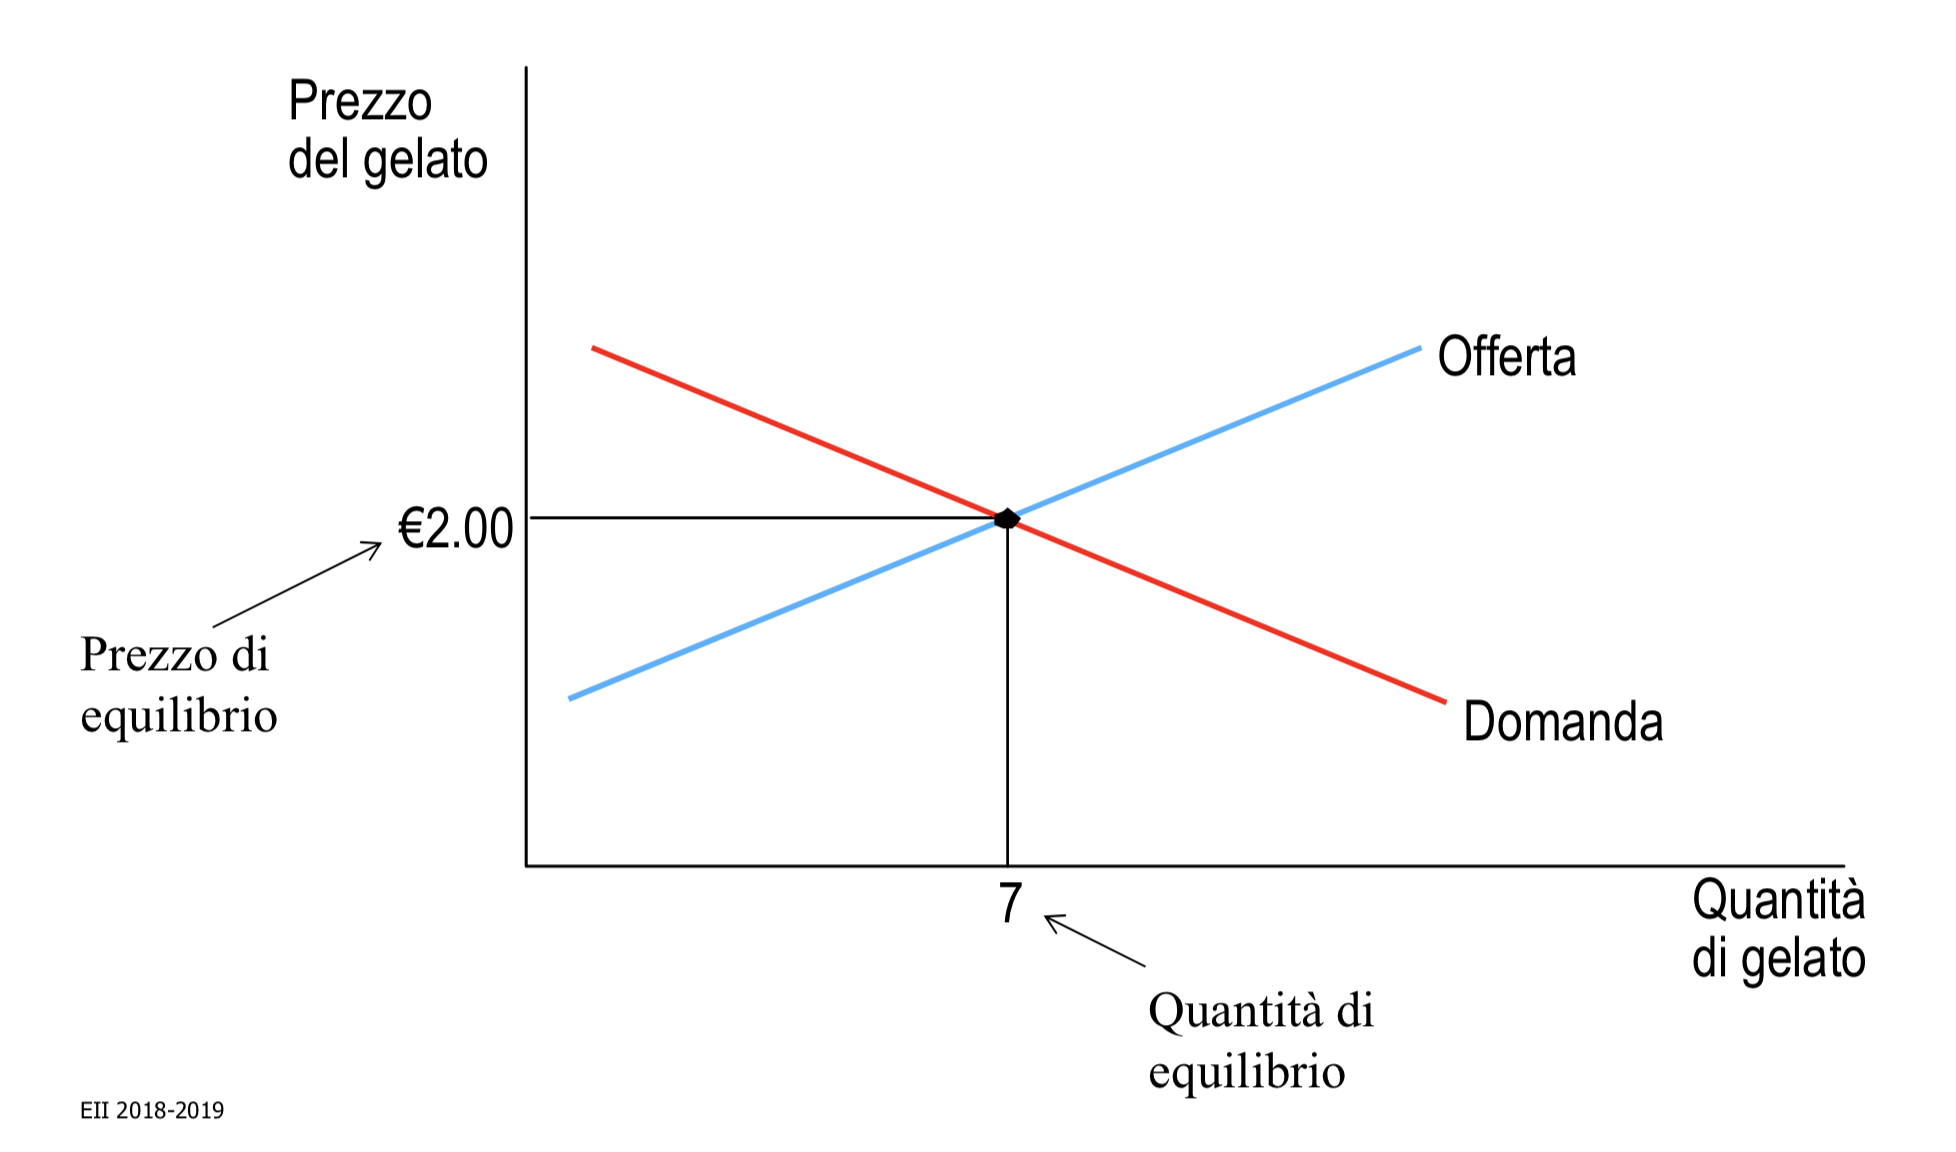
\includegraphics[width=0.7\linewidth]{forbice-marshalliana}
		\caption[Forbice marshalliana]{Forbice marshalliana}
		\label{fig:forbice-marshalliana}
	\end{figure}
	\section{Il disequilibrio}
	Si ha un eccesso di offerta quando la quantita' offerta e' maggiore di quella domandata, ovvero quando il prezzo di mercato e' piu' alto del prezzo di equilibrio e quindi i produttori non riescono a vendere tutto a quel prezzo.
	\medskip \\
	SI ha invece un eccesso di domanda quando la quantita' domandata e' maggiore di quella offerta, ovvero quando il prezzo di mercato e' piu' basso del prezzo di equilibrio e quindi i consumatori non riescono ad acquistare tutto a quel prezzo.
	\subsection{Due tipi di aggiustamento}
	\subsubsection{Approccio walrasiano}
	Il disequilibrio e' differenza nelle quantita' e segnala la presenza di un prezzo troppo alto/basso. Si raggiunge l'equilibrio variando il prezzo.
	\subsubsection{Approccio marshalliano}
	Il disequilibrio e' differenza tra prezzo d'acquisto e prezzo di vendita e segnala la presenza di una quantita' offerta troppo alta/bassa. Si arriva all'equilibrio variando la quantita'.
	\medskip \\L'approccio walrasiano e' piu' semplice ma ha il problema istituzionale di chi fissa il prezzo di partenza; l'approccio marshalliano e' invece piu' realistico.
	\section{La clausola \textit{ceteris paribus}}
	Espressione impiegata dagli economisti per indicare che in una certa analisi tutte le variabili diverse da quelle in oggetto sono ipotizzate costanti. Clausola alla base del metodo di equilibrio parziale, dove si studia un singolo mercato in isolamento
\end{document}
